\documentclass[12pt]{article}
\usepackage{amsmath,amsfonts, epsfig}
\usepackage{booktabs} % for better table formatting
\usepackage[authoryear]{natbib}
\usepackage{array}
\usepackage{multirow}
\usepackage{graphicx}
\usepackage{fancyhdr}
\usepackage{bm}
\pagestyle{fancy}
\lfoot{\texttt{ematm0067.github.io} / \texttt{ematm0044.github.io}}
\lhead{Introduction to AI - 02.4\_logistic - Conor}
\rhead{\thepage}
\cfoot{}

\usepackage{tikz}
\usetikzlibrary{positioning}

\usepackage{ifthen}
\newboolean{nopics}
\setboolean{nopics}{true}


\begin{document}

\section*{Logistic regression.} 

Lets begin with an example, the Canadian linguist Jack Chambers is
interested in dialect and language change among English speakers in
the eastern part of Canada. He did a broad study where he discovered
many on-going changes and tried to interpret them. The data are
available, at least in summary form at
\texttt{dialect.topography.artsci.utoronto.ca/}. In one example, from
what is called the Golden Horseshoe, which extends along the western
shore of Lake Ontario and includes the cities of Hamilton and Toronto,
he discovered what to me looks like a surprising shift from weak to
strong participle for the word \textsl{sneak}. He asked participants which they say from
\begin{itemize}
\item The little devil sneaked into the theatre.
\item The little devil snuck into the theatre.
\end{itemize}
and roughly speaking found that younger people prefer `snuck' to
`sneaked', the so called strong form over the weak. I had assumed
there was a general trend towards weak forms.

This graph below gives a simulated version of his data; the actual
data have more points but bundle the participants into age bands. For
the convenience of this lesson I have made artificial data, with fewer
points but where the ages take any whole-year value: the artificial
data is designed to have the same broad statistical structure as the
real data. In the graph age is plotted along the bottom, and the
$y$-value is zero for participants who say they use `snuck' and one
for those who use `sneaked'. A small jitter has been added to the $y$
value to stop the points covering each other, this is a common and
useful graphical device used for data like this.
\begin{center}
  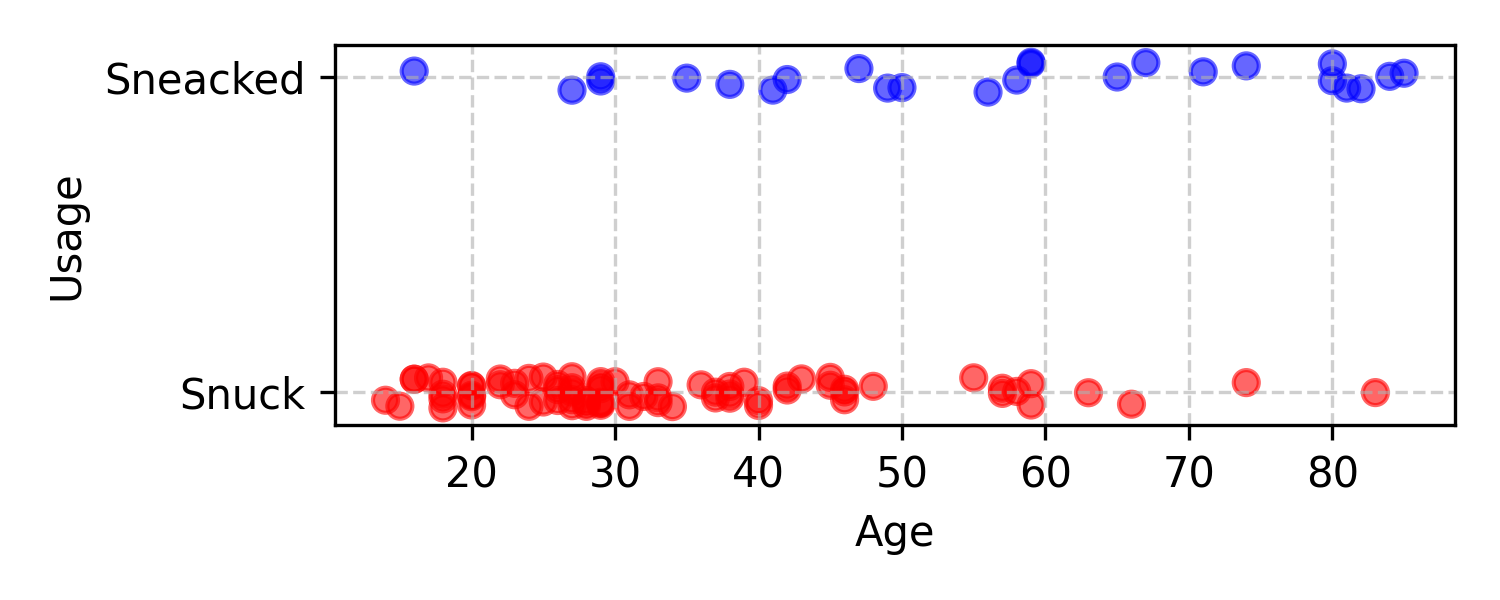
\includegraphics[]{02.4_sneak.png}
\end{center}

  Now, clearly there is some relationship between age and usage. If we
  take these data and bin them in ten year age bands and calculating
  for each band what fraction for each band says `sneaked' we get
  this:
\begin{center}
  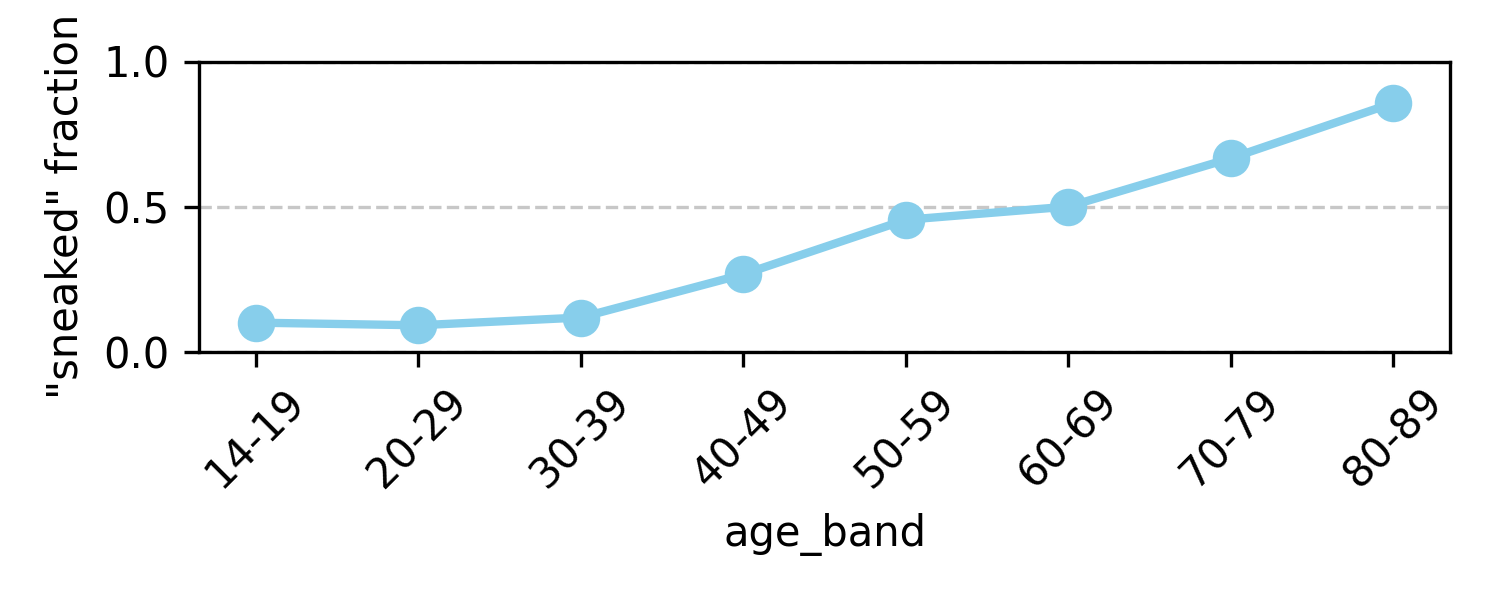
\includegraphics[]{02.4_fraction.png}
  \end{center}
  and it is clear that younger people say `snuck' more often than
  older. However, what we have learned so far is to model
\begin{equation}
\hat{u}=\beta_1 a+\beta_0
\end{equation}
where $a$ is the age and $u$ is some measure of
`snuck-saying-ness'. This, though, clearly does not work; partly
because a line looks to be the wrong shape but mostly because there is
a sort of category error. The data are not composed of quantitative
measurements of `snuck-saying-ness', the individual participants are
either `snuck' or `sneaked' and so the best measure of
`snuck-saying-ness' must surely be a probability, the probability a
participant will answer `snuck'. However $\hat{u}$ above does not look
much like a probability: it isn't limited to values between zero and
one.

At its simplest the idea behind logistic regression is to take
$\beta_1a+\beta_0$ and then use another function to `squash' it so
that the values are between zero and one, so
\begin{equation}
\hat{p}=f(\beta_1 a+\beta_0)
\end{equation}
where $f:\mathbb{R}\rightarrow[0,1]$ and
\begin{equation}
\hat{p_i}=f(\beta_1 a)i+\beta_0)
\end{equation}
is not the estimated probability that someone aged $a_i$ will prefer
`snuck'. One example of a function that does this is the logistic
function, often denoted using a sigma:
\begin{equation}
  \sigma(x)=\frac{1}{1+e^{-x}}
\end{equation}
which looks like this
\begin{center}
  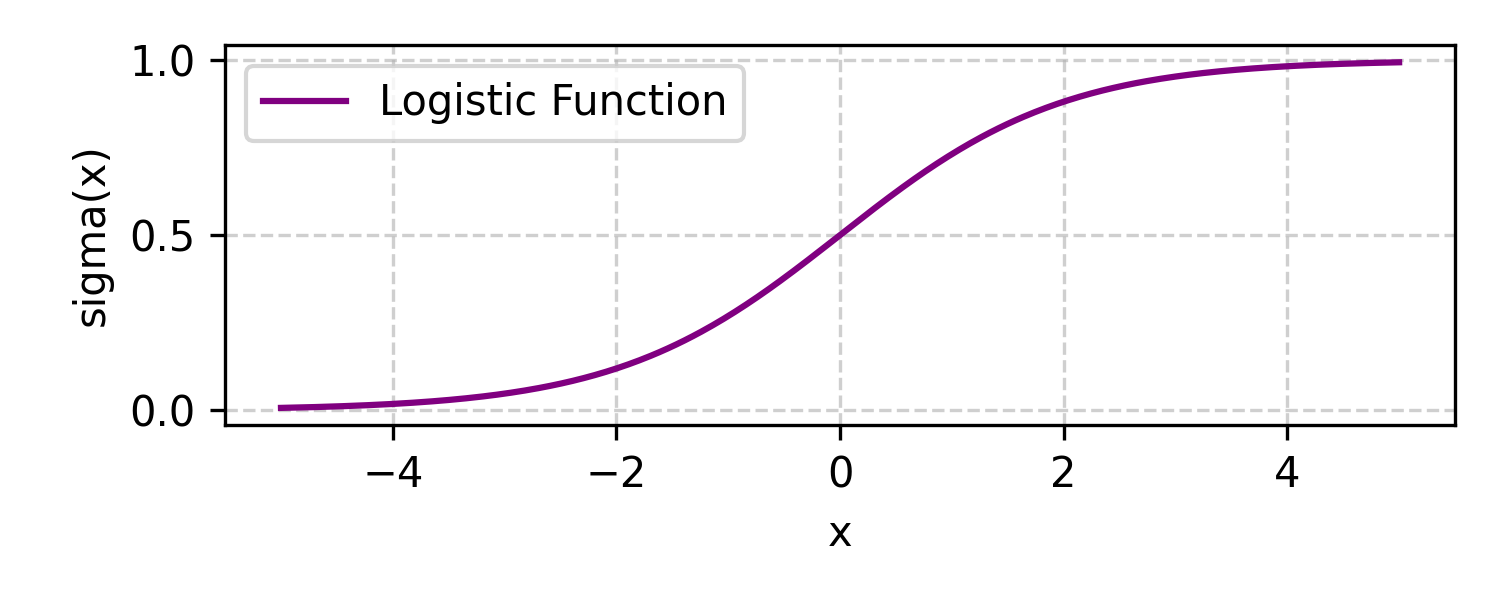
\includegraphics[]{02.4_logistic.png}
\end{center}
This isn't the only function that looks like this; there are lots of
others, we will discuss why this particular example is chosen
later. In general, a function that has this general shape is called a
\textsl{sigmoid function} and other examples include the arctan. A
function wrapped around a linear model in regression is often called a
\textsl{link function}.

First, lets consider as to how we should fix $\beta_0$ and
$\beta_1$. For now lets move away from the specific example and use
the more general terminology of `success' and `failure' for the
trials, equivalent to choice of `snuck' and `sneaked' and imagine we
have a model
\begin{equation}
\hat{p}(x)=\sigma(\beta_1 x+\beta_0)
\end{equation}
so $p(x_i)$ is the `true probability' for success when $x=x_i$ and out
estimate for the probability is $\hat{p}(x_i)$.  Given some data, we
are interested in how well the estimated probabilities predict the
actual results. This leads to the important concept of
\textsl{likelihood}, A good model makes the data `likely', that is, it
assigns it a probability near one. It sort of flips everything on its
head, rather than a probability giving the chance of something
happening, we already have the data and we want a model whose
probability is high for what we know actually happened! This sort of
logical somersault is often the key to machine learning concepts!

Anyway, if a data point at $x_i$ is a success the likelihood is
$\hat{p}(x_i)$, if it is a failure, then the likelihood is
$1-\hat{p}(x_i)$.
For a set of data
\begin{equation}
  \mathcal{D}=\{(x_1,y_1),(x_2,y_2),\ldots,(x_n,y_n)\}
\end{equation}
where $y_i=1$ for success and $y_1=0$ for failure, the overall
likelihood is
\begin{equation}
  L=\prod_{y_i=1}\hat{p}(x_i)\prod_{y_i=0}(1-\hat{p}(x_i))
\end{equation}
The goal is to pick the parameters in the definition of $\hat{p}$ to
maximize $L$.

Now one problem is probabilities is that they get
multiplied; this causes no end of grief, for a start, it can make the
calculus very tedious and, more seriously, multiplying lots of small
numbers gives you a tiny number and this can cause imprecision
problems with numerical computation. For these reasons alone it makes
sense to consider the log-likelihood, recalling
\begin{equation}
  \log{ab}=\log{a}+\log{b}
\end{equation}
we have
\begin{equation}
  \log{L}=\sum_{y_i=1}\log\hat{p}(x_i)+\sum_{y_i=0}\log(1-\hat{p}(x_i))
\end{equation}
or, sometimes we use $-\log{L}$, the negative log-likelihood, purely
because we like to minimize things rather than maximize them, even if
one is equivalent to the other. I should also say that adding the
logarithm makes good sense computationally and, as with using the
square mean error rather than the root mean square error, the fact
that the logarithm is a monotonically increasing function means that
we aren't changing where the maximimum is, so it could just be
considered a matter of convenience. However, while we won't go into it
here, there are also strong arguments from information theory to use
the logarithm.

Hence, in short, we have a model mapping data to estimated
probabilities, we can write this as $\hat{p}(x;\theta)$ where $\theta$
are the parameters, in this case $\beta_0$ and $\beta_1$. Our goal is
to pick the values of $\beta_0$ and $\beta_1$ to minimize the
objective function, in this case the negative log-likelihood,
sometimes in this case somewhat sloppily referred to as the
cross-entropy loss. In the notation used in machine learning we want
\begin{equation}
  \theta_*=\text{argmin}_\theta [-\log{L(\text{data},\theta)}]
\end{equation}
Here $\theta_*$ is a common notation for `the best value' or `the
value we are looking for' and argmin$_\theta$[stuff] is the value of
$\theta$ which minimizes `stuff'.

Now we need to do some calculus. Lets get the little pieces we
need. Using the quotient rule you can check
\begin{equation}
  \frac{d\sigma{x}}{dx}=\sigma(x)[1-\sigma(x)]
\end{equation}
and you should recall that
\begin{equation}
  \frac{d\log{x}}{dx}=\frac{1}{x}
\end{equation}
So, using the chain rule
\begin{equation}
  \frac{d}{d\beta_0}\log{\sigma(\beta_1x+\beta_0)}=1-\sigma(\beta_1x+\beta_0)
\end{equation}
and
\begin{equation}
  \frac{d}{d\beta_1}\log{\sigma(\beta_1x+\beta_0)}=x[1-\sigma(\beta_1x+\beta_0)]
\end{equation}
In fact, putting this together, along with the two similar derivatives, we find
\begin{align}
  \frac{d\log{\hat{p}}}{d\beta_0}&=1-\hat{p}\\  \nonumber
    \frac{d\log{\hat{p}}}{d\beta_1}&=x(1-\hat{p})\\ \nonumber
  \frac{d\log{(1-\hat{p})}}{d\beta_0}&=\hat{p}\\ \nonumber
  \frac{d\log{(1-\hat{p})}}{d\beta_1}&=x\hat{p}
\end{align}
Clearly the logistic function is very convenient but not convenient
enough for a closed form solution. These formula mean that the
derivatives of the negative log-likelihood will contain terms that
look like $\sigma(\beta_1x_i+\beta_0)$ for the different $x_i$
values. This will lead to equations where you can't write down a
general solution, as we could with linear regression. However, the
numerical problem, for example using gradient descent as described
before, can find a solution.

As a side note, any library for data modelling will have a command for
doing logistic regression; this will find the values of the beta
parameters using numerical methods. This is a quick and robust
operation, the objective function has a nice structure and there is an
explicit formula for the gradient based on the derivatives above. In
fact, although gradient descent will work in this case, there is
enough known that other, quicker and more bullet-proof, methods are
usually employed, such as the Newton-Raphson algorithm. This algorithm
will solve the equations for zero gradient rather than navigating down
the gradient. Gradient descent is commonly used because it can
commonly be applied, but it is not particularly quick and it can be
fussy so in special cases where there are alternatives it is usually
best to use them. Luckily a lot of these implementation details are
hidden away from us by software libraries!

Returning to our example we can fit the logistic curve, we find $\beta_0=-4.03$ and $\beta_1= 0.067$, it looks like this:
\begin{center}
  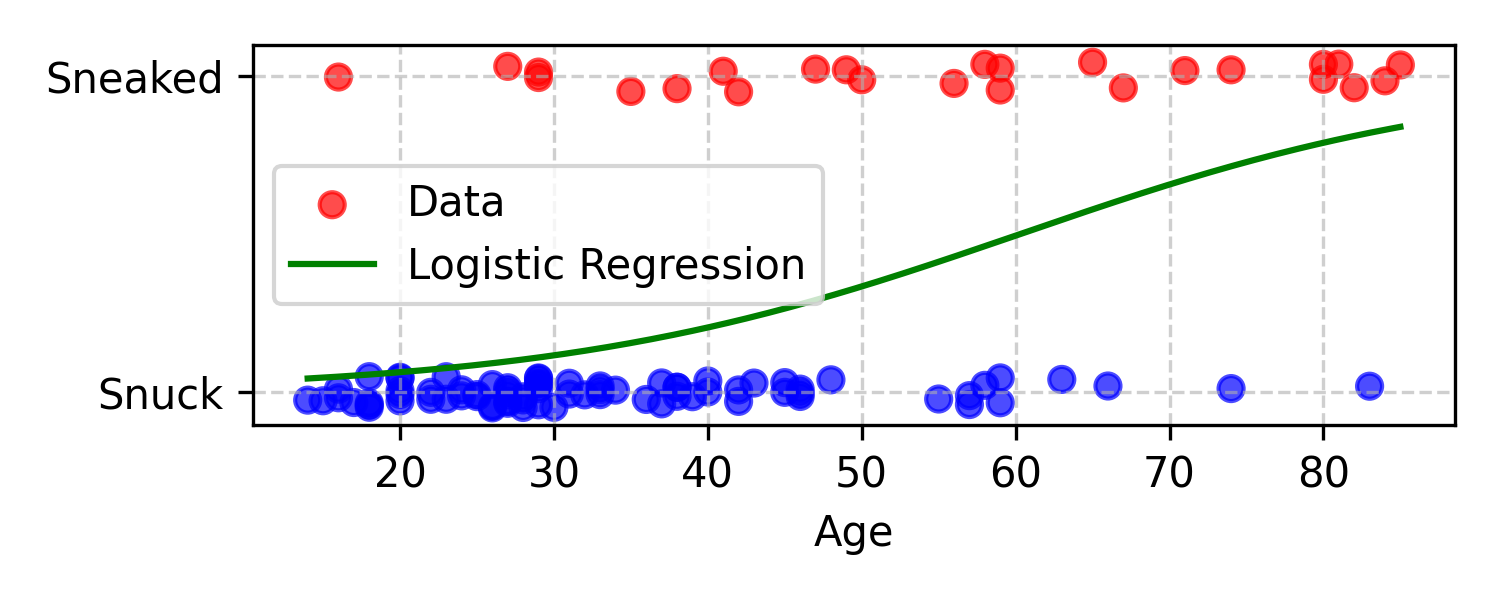
\includegraphics[]{02.4_fit.png}
  \end{center}
We can see that there is a nice fit. The data are from twenty years
ago, you could imagine replacing the age with date of birth to use
this curve to make predictions about how people speak today. In
performed an undersampled study, well to be more honest I asked
exactly one person from the Golden Horseshoe what they would say and
the said ``snuck'' for sure, that they were aware of `sneaked' as an
alternative but it seemed very old-fashioned.

Logistic regression is one of the basic tools of data science and is
with great frequency a useful approach to data. Our discussion has not
really addressed the question as to why it works; we have defined a model:
\begin{equation}
  \hat{p}(x,\beta_0,\beta_1)=\sigma(\beta_1x+\beta_0)
\end{equation}
and discussed how to fit it, we have also seen it is the right sort of
model for data with a yes or no outcome. This does not tell us that we
can expect it to work, no more than our discussion of linear
regression explained why it is often useful. This, of course, is a
complicated question; in the case of linear regression we can point to
the frequency of linear rules in nature and to the prominence of the
linear term in a Taylor expansion; we can also point to the imperical
fact that it often works. In the case of logistic regression the
discussion is even more complicated because we need to also account
for the particular form of the logistic function.

In fact, there is a sort of attempt at a principled argument given
which looks something like this, if
\begin{equation}
  \hat{p}=\frac{\hat{o}}{\hat{o}+1}
\end{equation}
where in the model
\begin{equation}
  \hat{o}=e^{\beta_1x+\beta_0}
\end{equation}
where you should note the sign of the exponent. Now solving for $o$ we get
\begin{equation}
  \hat{o}=\frac{\hat{p}}{1-\hat{p}}
\end{equation}
This ratio is known as the \textsl{odds}, the ratio of the probability
of success to the probability of failure. In terms of the odds, the
regression model is stating that
\begin{equation}
  \log\hat{o}=\beta_1x+\beta_0
\end{equation}
In other words, the assumption in logistic regression is that the
log-odds depends in a linear way on the variable $x$. If you look you
will find arguments as to why this is a natural assumption, if you
understand these arguments come and explain them to me, I find them a
bit mysterious, but the key idea is that a lot of processes that
produce yes or no type data are well approximated by assuming there is
a linear model for the log-odds. My own feeling is that the precise
choice of a sigmoid function does not really matter, the link to
log-odds is elegant but does not give a simple proof that the logistic
function is the `best' sigmoid function; however, the calculus works
out nicely using the logistic function and imperically we know
logistic regression is often useful!

As a final note, obviously everything we've done here has relied on a
one-dimensional regression:
\begin{equation}
  \hat{p}=\sigma(\beta_1x+\beta_0)
\end{equation}
but in practice you will usually have more than one independent
variable and the whole framework generalizes in the obvious way:
\begin{equation}
  \hat{p}=\sigma(\bm{\beta}\cdot \mathbf{x}+\beta_0)
\end{equation}


\section*{Summary}
Lots of data has the form $(\mathbf{x},y)$ where $\mathbf{x}$ are
independent variables and $y$ the outcome has a binary form, yes or
no, zero or one, failure of success. A common model for this is logistic regression
\begin{equation}
  \hat{p}=\sigma(\bm{\beta}\cdot \mathbf{x}+\beta_0)
\end{equation}
where $\sigma(x)=1/(1+\exp{(-x)})$ is the logistic function. To find the parameters we usually minimize the negative log-likelihood.
\begin{equation}
  \mathcal{E}=-\log{L}=-\sum_{y_i=1}\log\hat{p}(\mathbf{x}_i)-\sum_{y_i=1}\log[1-\hat{p}(\mathbf{x}_1)]
\end{equation}
This is done numerically.
\end{document}

